\subsubsection{Kürzester Weg finden}

Da es nur 8 Knoten im Graph gibt, wurde von Anfang an vermutet, dass die Geschwindigkeit des Algorithmus vernachlässigt werden kann.

Um zu überprüfen, dass diese These stimmt, wurde ein traditioneller Dijkstra Algorithmus in Python implementiert. Dabei wurde von einem Knoten den kürzesten Weg zu allen anderen Knoten im vorgegebenen Graphen berechnet. währenddessen wurde die Zeit für die Berechnungen gestoppt. Um Hardware Einflüsse zu minimieren, wurde dieses Skript auch auf einem Single-Board Computer, namentlich einem Raspberry Pi 4 (4GB) ausgeführt, und einige male wiederholt. Was uns zu nachfolgender Ausgabe und Kenntnissen bringt:

\begin{figure}[H]
\begin{subfigure}{0.275\textwidth}
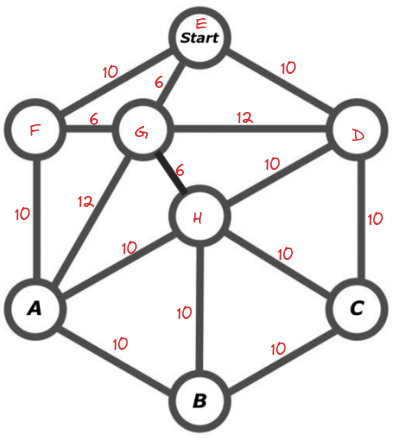
\includegraphics[width=0.95\linewidth]{img/graph_with_weighted_edges.png} 
\caption{Gewichteter Graph}
\label{fig:weighted-graph}
\end{subfigure}
\begin{subfigure}{0.720\textwidth}
\begin{footnotesize}
\begin{verbatim}
Shortest distance from E to A is 18 via path: E -> G -> A
Shortest distance from E to B is 22 via path: E -> G -> H -> B
Shortest distance from E to C is 20 via path: E -> D -> C
Shortest distance from E to D is 10 via path: E -> D
Shortest distance from E to E is 0 via path: E
Shortest distance from E to F is 10 via path: E -> F
Shortest distance from E to G is 6 via path: E -> G
Shortest distance from E to H is 12 via path: E -> G -> H
This calculation took about 0.128ms
\end{verbatim}
\end{footnotesize}
\caption{Skript Ausgabe}
\label{fig:djikstra-test-skript-output}
\end{subfigure}

\caption{Djikstra Algoritmus Test mit Python}
\label{fig:djikstra-test-output}
\end{figure}

Um den kürzesten Pfad achtmal zu berechnen, wurden etwa 0,128 ms benötigt, was ausreichend schnell ist. Aufgrund dieses Tests wurde entschieden, einen selbst implementierten, einfachen Dijkstra-Algorithmus zu verwenden, da es wichtig ist, dass der Algorithmus möglichst leichtgewichtig ist, da nur begrenzte Rechenleistung und Speicher zur Verfügung stehen.

Das Skript wurde in einem Github Gist veröffentlicht und ist unter folgendem Link aufrufbar: \url{https://gist.github.com/dimschlukas/2632116f913b1e10eea9be40e62b2630}

\subsubsection{Winkelerkennung}\label{winkelerkennung}

Um die Winkel der abgehenden Kanten eines Knoten zu detektieren, macht unser Roboter vor dem Befahren eines Knotens ein Bild dessen. Dazu ist jedoch zu beachten, wie in Kapitel PLACEHOLDER beschrieben, wird unsere Kamera in einem Winkel von PLACEHOLDER Grad montiert. So können wir naheliegende Knoten vor dem Roboter, wie auch weit entfernte Pylonen in einem Bild erkennen, ohne die Kamera schwenken zu müssen.
Da wir dadurch nun aber verzerrte Bilder aufzeichnen, muss an dem Bild zuerst einer geometrische Transformation durchgeführt werden. Sodass wir schlussendlich ein verzerrungsfreihe Ansicht auf den Knoten haben. Anschliessend können die einzelnen Winkel ohne Probleme durch mathematische Formeln berechnet werden.

Nachfolgend wird dies Schritt für Schritt nachvollziehbar dargestellt:

\begin{enumerate}
    \item Vor dem Knoten anhalten und Bild aufnehmen
    \begin{figure}[H]
        \centering
        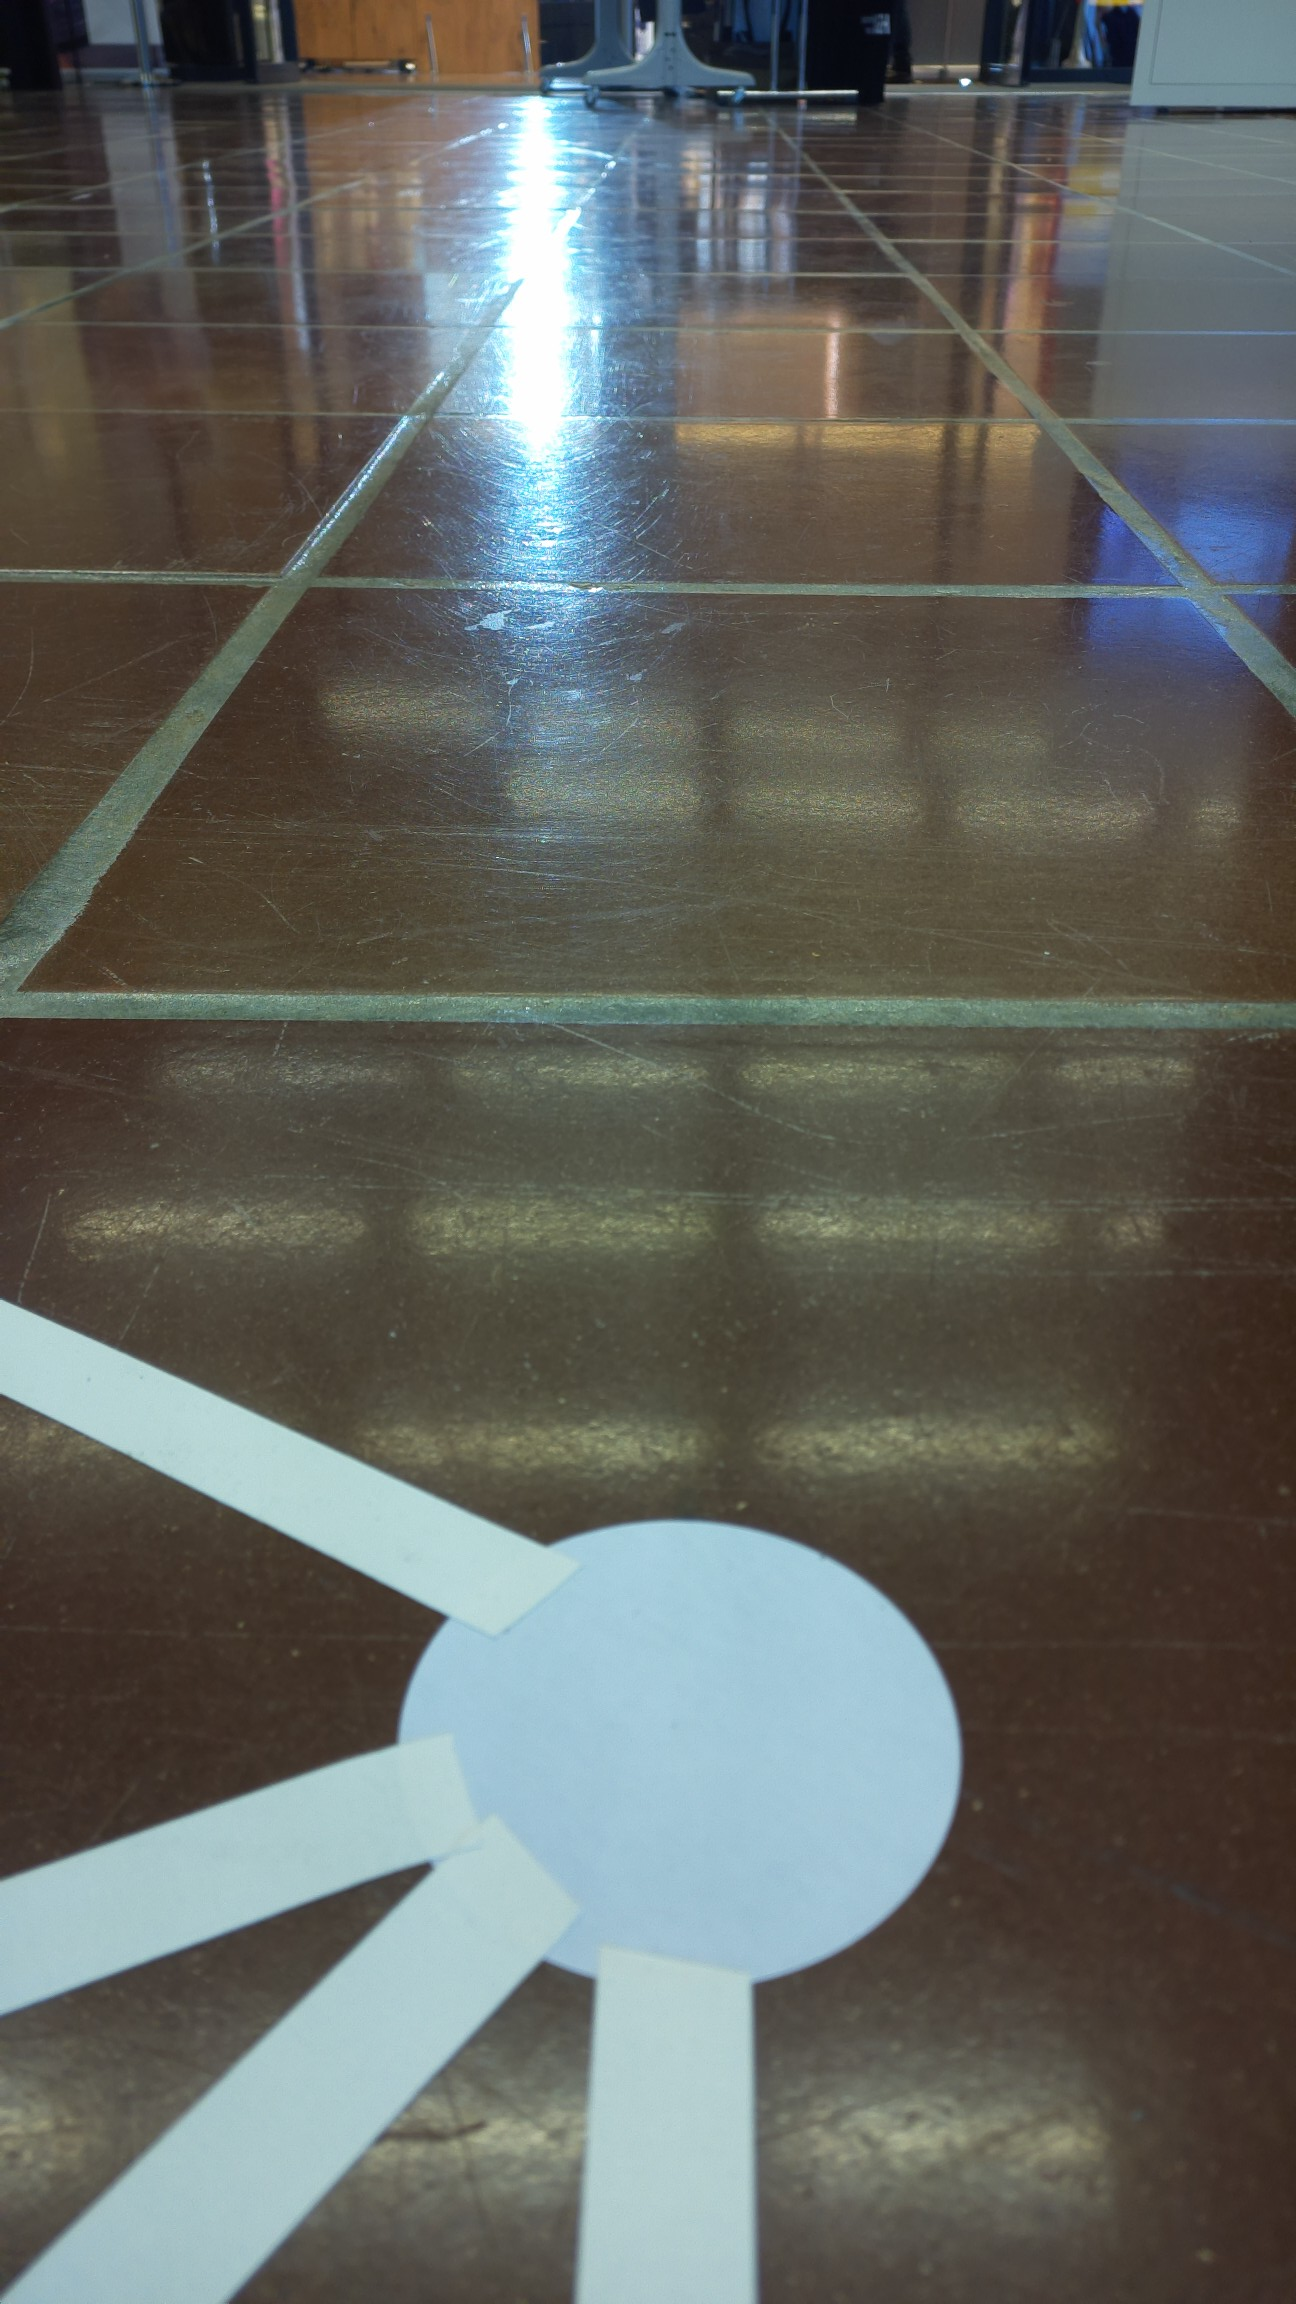
\includegraphics[width=0.5\linewidth, angle=90]{assets/informatik-prototyp/opencv/angle_detection/image_taken_by_pi_camer_before_node.jpg}
        \caption{Kameraaufnahme eines Knotens}
        \label{fig:enter-label}
    \end{figure}
    \item Geometrische Transformation anhand fix definierten Punkten anwenden
    \item Knoten sowie dessen Mittelpunkt detektieren
    \item Ausgehende Kanten detektieren
    \item Geometrischer Schwerpunkt der einzelnen Kanten detektieren.
    \item Winkel der Kanten berechnen
\end{enumerate}

PLACEHOLDER
Winkel messunge, Bildverzerrung, Tests wieso 20cm abstand
TODO Beschreib Winkel messen \& verzerren genauer im Prototyp

Wie Winkel intern abspeichern, wie mapping, ...

Offset 180 Grad


Hardcoded Winkel, simuliere gemessene Winkel und reageire, Mapping und speichern

\subsubsection{Graph-, Pylonen- und Barrierenerkennung}

% \textbf{Spiegelung}

% Starke Spiegelungen stellen ein grosses Problem bei der Erkennung von Knoten dar. Um die Bilder zu entspiegeln, können die Lichtverhältnisse angepasst, Polfilter verwendet oder Nachbearbeitungen durchgeführt werden.\cite{avoid-reflection}

% Beleuchtung

Als Basis fuer die Bilderkennung, wurde ein Graph aufgeklebt in der Mensa. Es wurden mehrere Bilder gemacht, wobei Pylonen und Barrieren willkuerlich auf Knoten und Kanten gestellt wurden und immer wieder verschoben wurden.

\textbf{FAST, SIFT}

PLACEHOLDER

\textbf{Objekterkennung mit OpenCV}

PLACEHOLER

\textbf{YOLOv11}

Auf Roboflow\footnote{https://roboflow.com/} wurden die insgesamt 39 erstellten Bilder labeled.
Das bedeutet, dass manuell die zu erkennenden Objekte ausgewaehlt und zu bestimmten Klassen hinzugefuegt wurden.

Danach wird das Datenset unterteilt in verschiedene Gruppen: Train, Validation, Test. Die Training Daten werden verwendet mit den Markierungen, damit das Model davon lernen kann. Das Validierungsset wird benoetigt, um waehrend dem Trainingsprozess zu pruefen, wie gut das Model ist und wie es angepasst werden soll. Das Testset wird schlussendlich verwendet, um zu testen, wie gut das angepasste Model die einzelnen Elemente erkennt. Dieses Testset ist noetig, weil es wichtig ist, dass die Daten, die schlussendlich verwendet werden, um zu pruefen, wie gut das Model ist, dem Model noch komplett unbekannt sein sollten.
\begin{figure}[H]
    \centering
    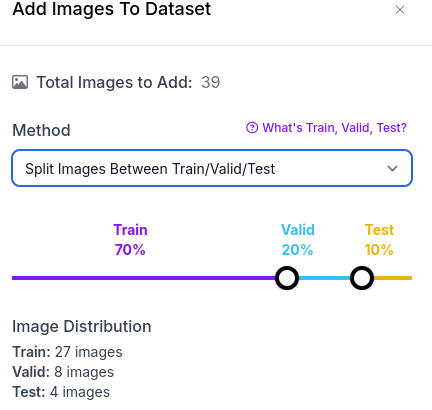
\includegraphics[width=0.5\linewidth]{assets/informatik-prototyp/yolo/train-test-split.png}
    \caption{Datenset Split}
    \label{fig:data-split}
\end{figure}

Als erstes wurden versucht ein Model zu trainieren, das alle Graphenelemente (Knoten und Kanten) und Hindernisse erkennt:

\begin{figure}[H]
\begin{subfigure}{0.55\textwidth}
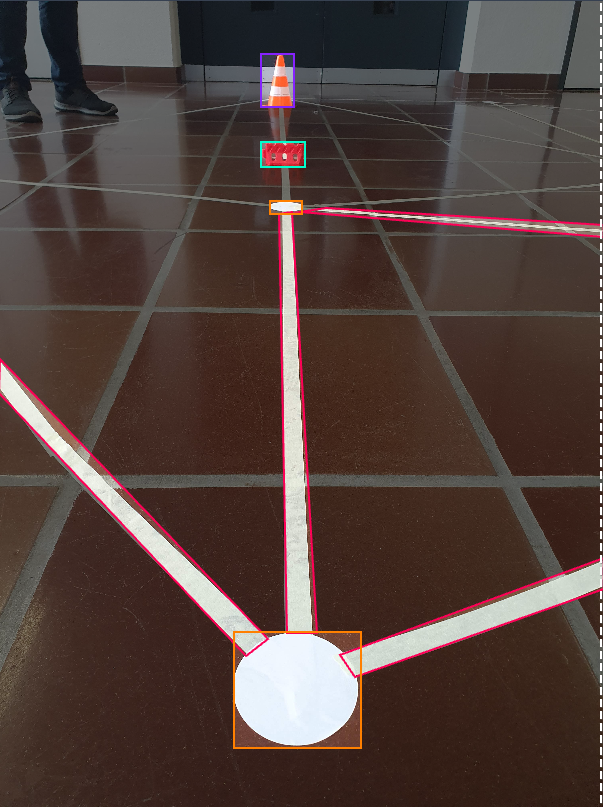
\includegraphics[width=0.95\linewidth]{assets/informatik-prototyp/yolo/labeled-image-lines.png} 
\caption{Bild mit Elementen + Linie markiert}
\label{fig:labeled-image-lines}
\end{subfigure}
\begin{subfigure}{0.4\textwidth}
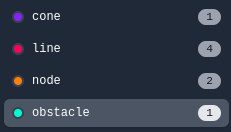
\includegraphics[width=0.95\linewidth]{assets/informatik-prototyp/yolo/labeled-classes-lines.png} 
\caption{Markierte Klassen mit Linie}
\label{fig:line-classes-lines}
\end{subfigure}

\caption{Roboflow labeled Bild mit Linien}
\label{fig:labeling-with-lines}
\end{figure}


Mihilfe eines Jupyter Notebooks, das von Roboflow zur Verfuegung gestellt wird, wurde ein YOLO Model mit 10 Epochs\footnote{https://deepai.org/machine-learning-glossary-and-terms/epoch} trainiert. Danach wurden Bilder aus dem Testset genutzt, wobei das Model versucht die einzelnen Elemente zu erkennen. Zusaetzlich wurde eine Confusion Matrix\footnote{https://www.sciencedirect.com/topics/engineering/confusion-matrix\#:\~:text=A\%20confusion\%20matrix\%20represents\%20the,by\%20model\%20as\%20other\%20class.} erstellt, die zeigt, welche Elemente als was erkannt wurde.

\begin{figure}[H]
\begin{subfigure}{0.3\textwidth}
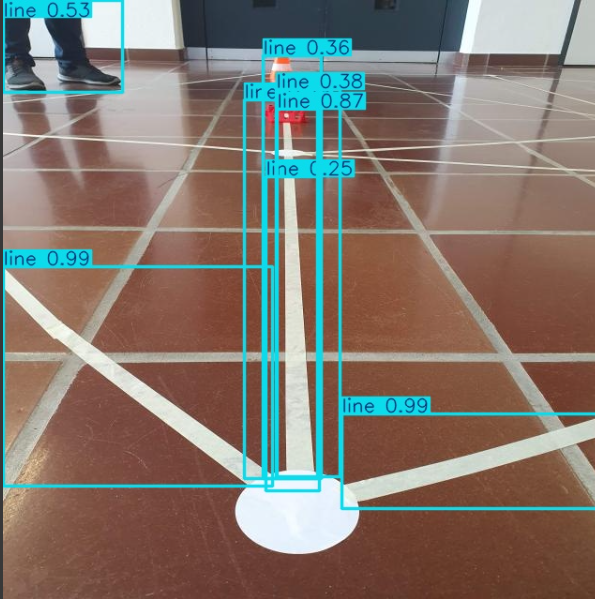
\includegraphics[width=0.95\linewidth]{assets/informatik-prototyp/yolo/line-recognitions.png} 
\caption{Erkanntes Bild mit Linien}
\label{fig:image-recognition-with-lines}
\end{subfigure}
\begin{subfigure}{0.69\textwidth}
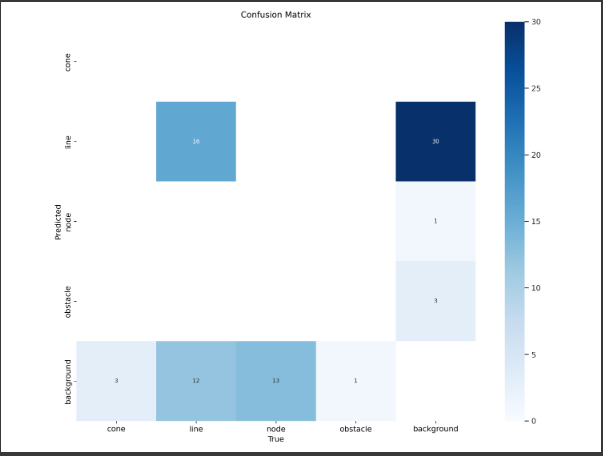
\includegraphics[width=0.95\linewidth]{assets/informatik-prototyp/yolo/conf-matrix-lines.png} 
\caption{Confusion Matrix mit Linien}
\label{fig:conf-matrix-lines}
\end{subfigure}

\caption{Bilderkennung inklusive Linien}
\label{fig:recognition-with-lines}
\end{figure}

Aus diesem Experiment war klar, sowohl aus dem Bild mit den "erkannten" Linien, als auch von der Confusion Matrix, dass Linien nicht korrekt erkannt werden koennen.
Aus der Confusion Matrix kann gelesen werden, dass von allen erkannten Linien in 4 Bildern, 30 Linien erkannt wurden an Stellen, an denen sich gar nichts befindet ("background").

Als naechste wurde das gleiche noch einmal durchgefuehrt. Dieses Mal wurde die Line-Klasse entfernt und es wurden nur noch Knoten, Pylonen und Barrieren markiert.

\begin{figure}[H]
\begin{subfigure}{0.55\textwidth}
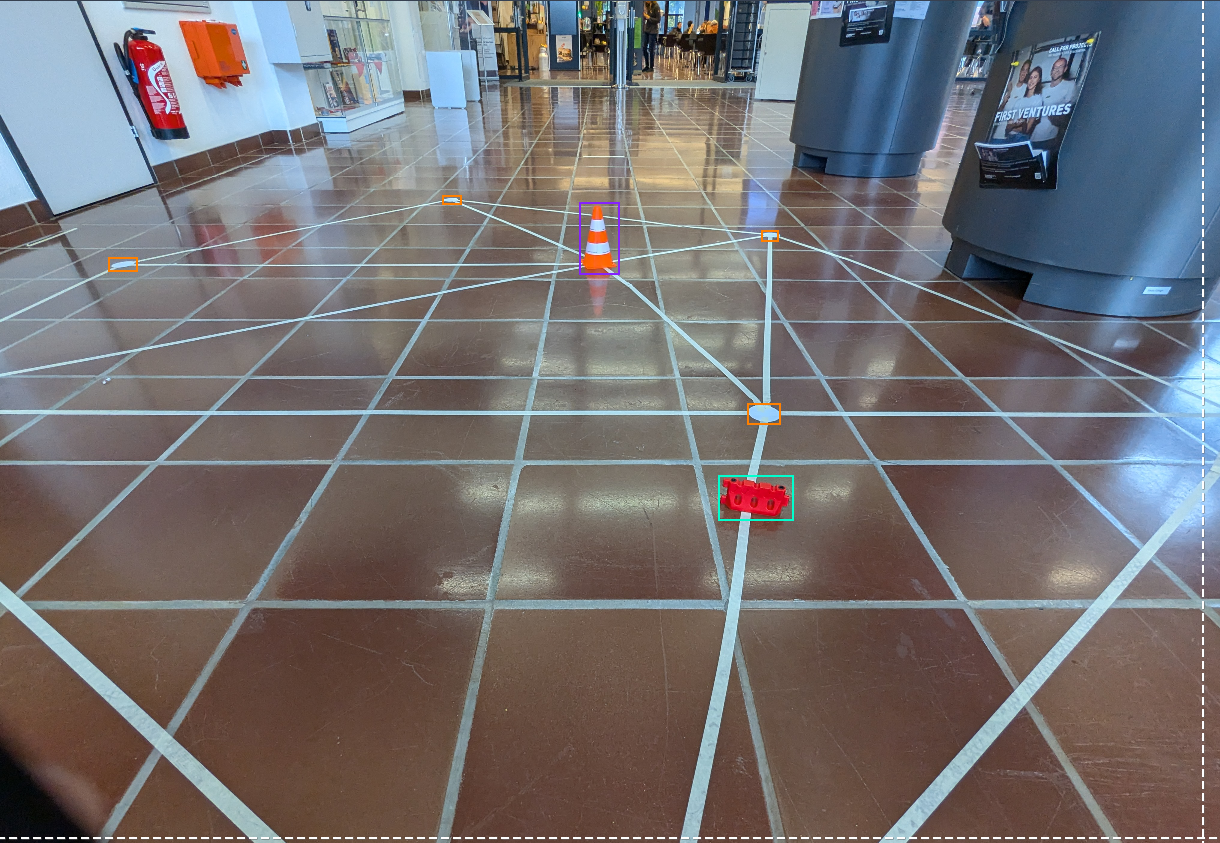
\includegraphics[width=0.95\linewidth]{assets/informatik-prototyp/yolo/labeled-image.png} 
\caption{Bild mit Elementen markiert}
\label{fig:labeled-image}
\end{subfigure}
\begin{subfigure}{0.4\textwidth}
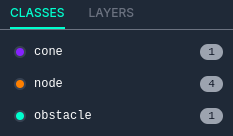
\includegraphics[width=0.95\linewidth]{assets/informatik-prototyp/yolo/labeled-classes.png} 
\caption{Markierte Klassen}
\label{fig:line-classes}
\end{subfigure}

\caption{Roboflow labeled Bild mit Linien}
\label{fig:labeling-with-lines}
\end{figure}

Die Bilderkennung des selben Jupyter Notbooks mit den reduzierten Klassen sah wie folgt aus:

\begin{figure}[H]
\centering
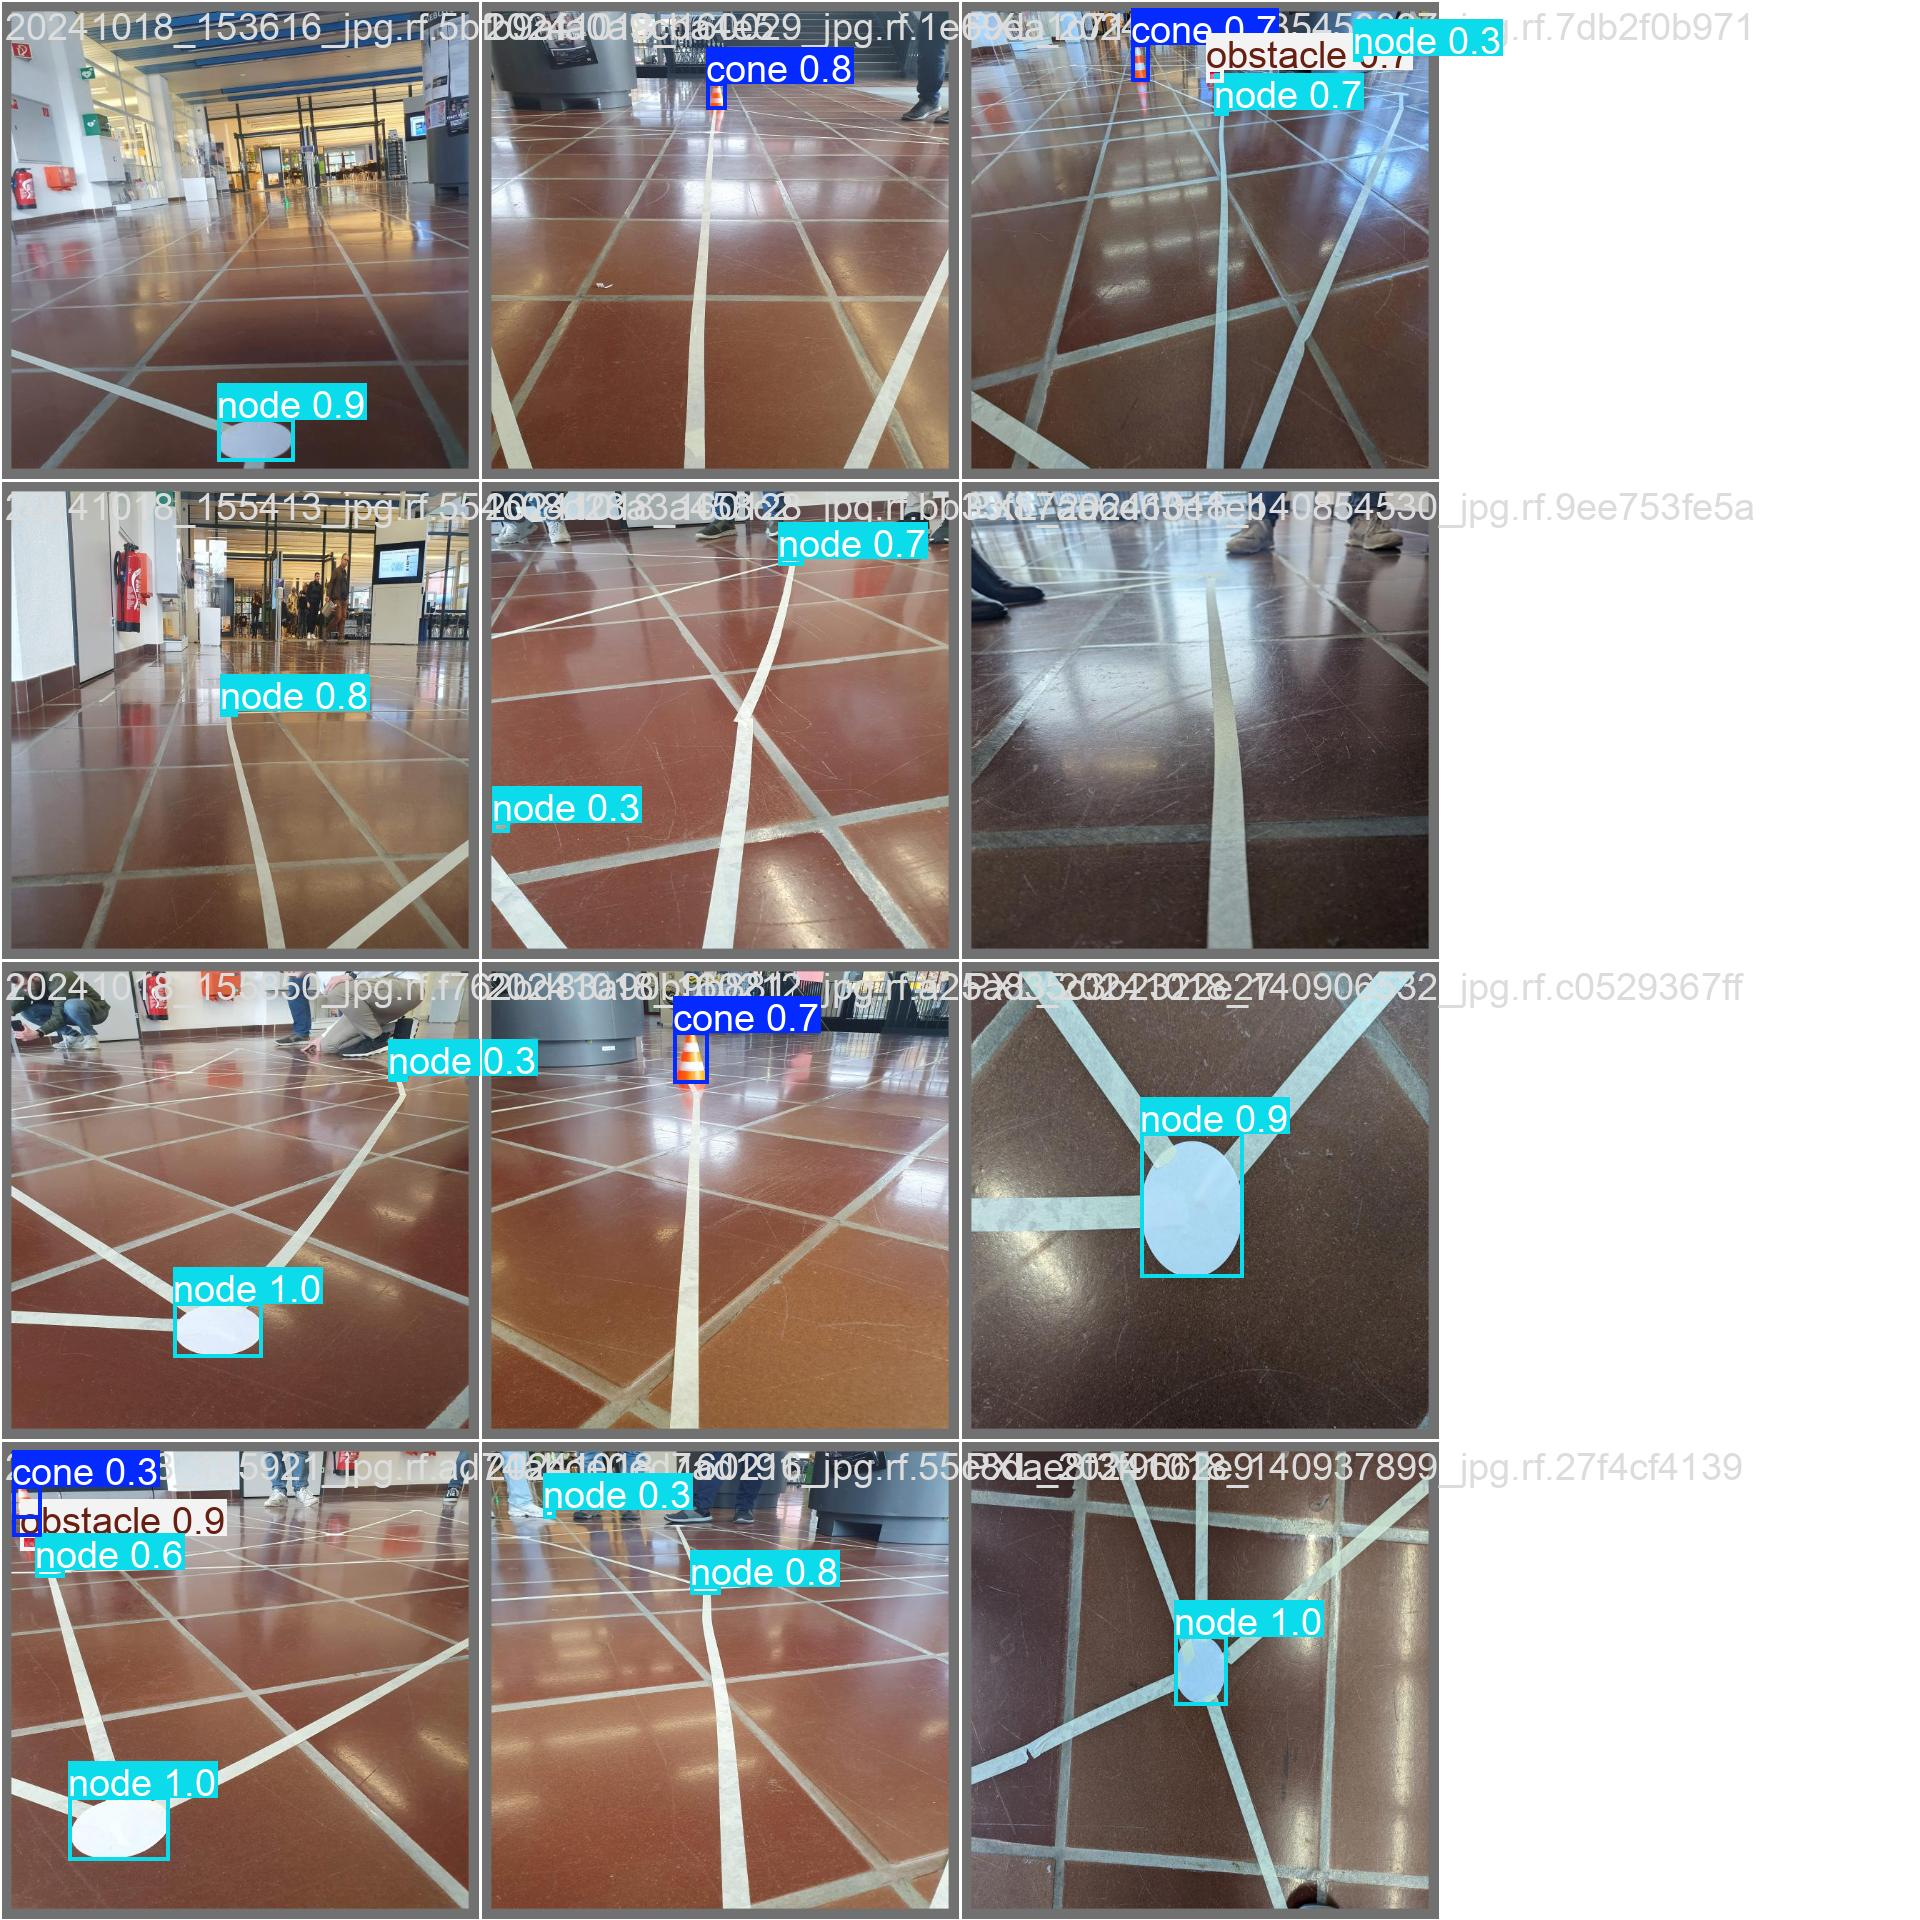
\includegraphics[width=\textwidth -30mm]{assets/informatik-prototyp/yolo/recognized-images.jpeg}
\caption{YOLOv11 Bilderkennung}
\label{fig:img-recognition-yolo}
\end{figure}

\begin{figure}[H]
\centering
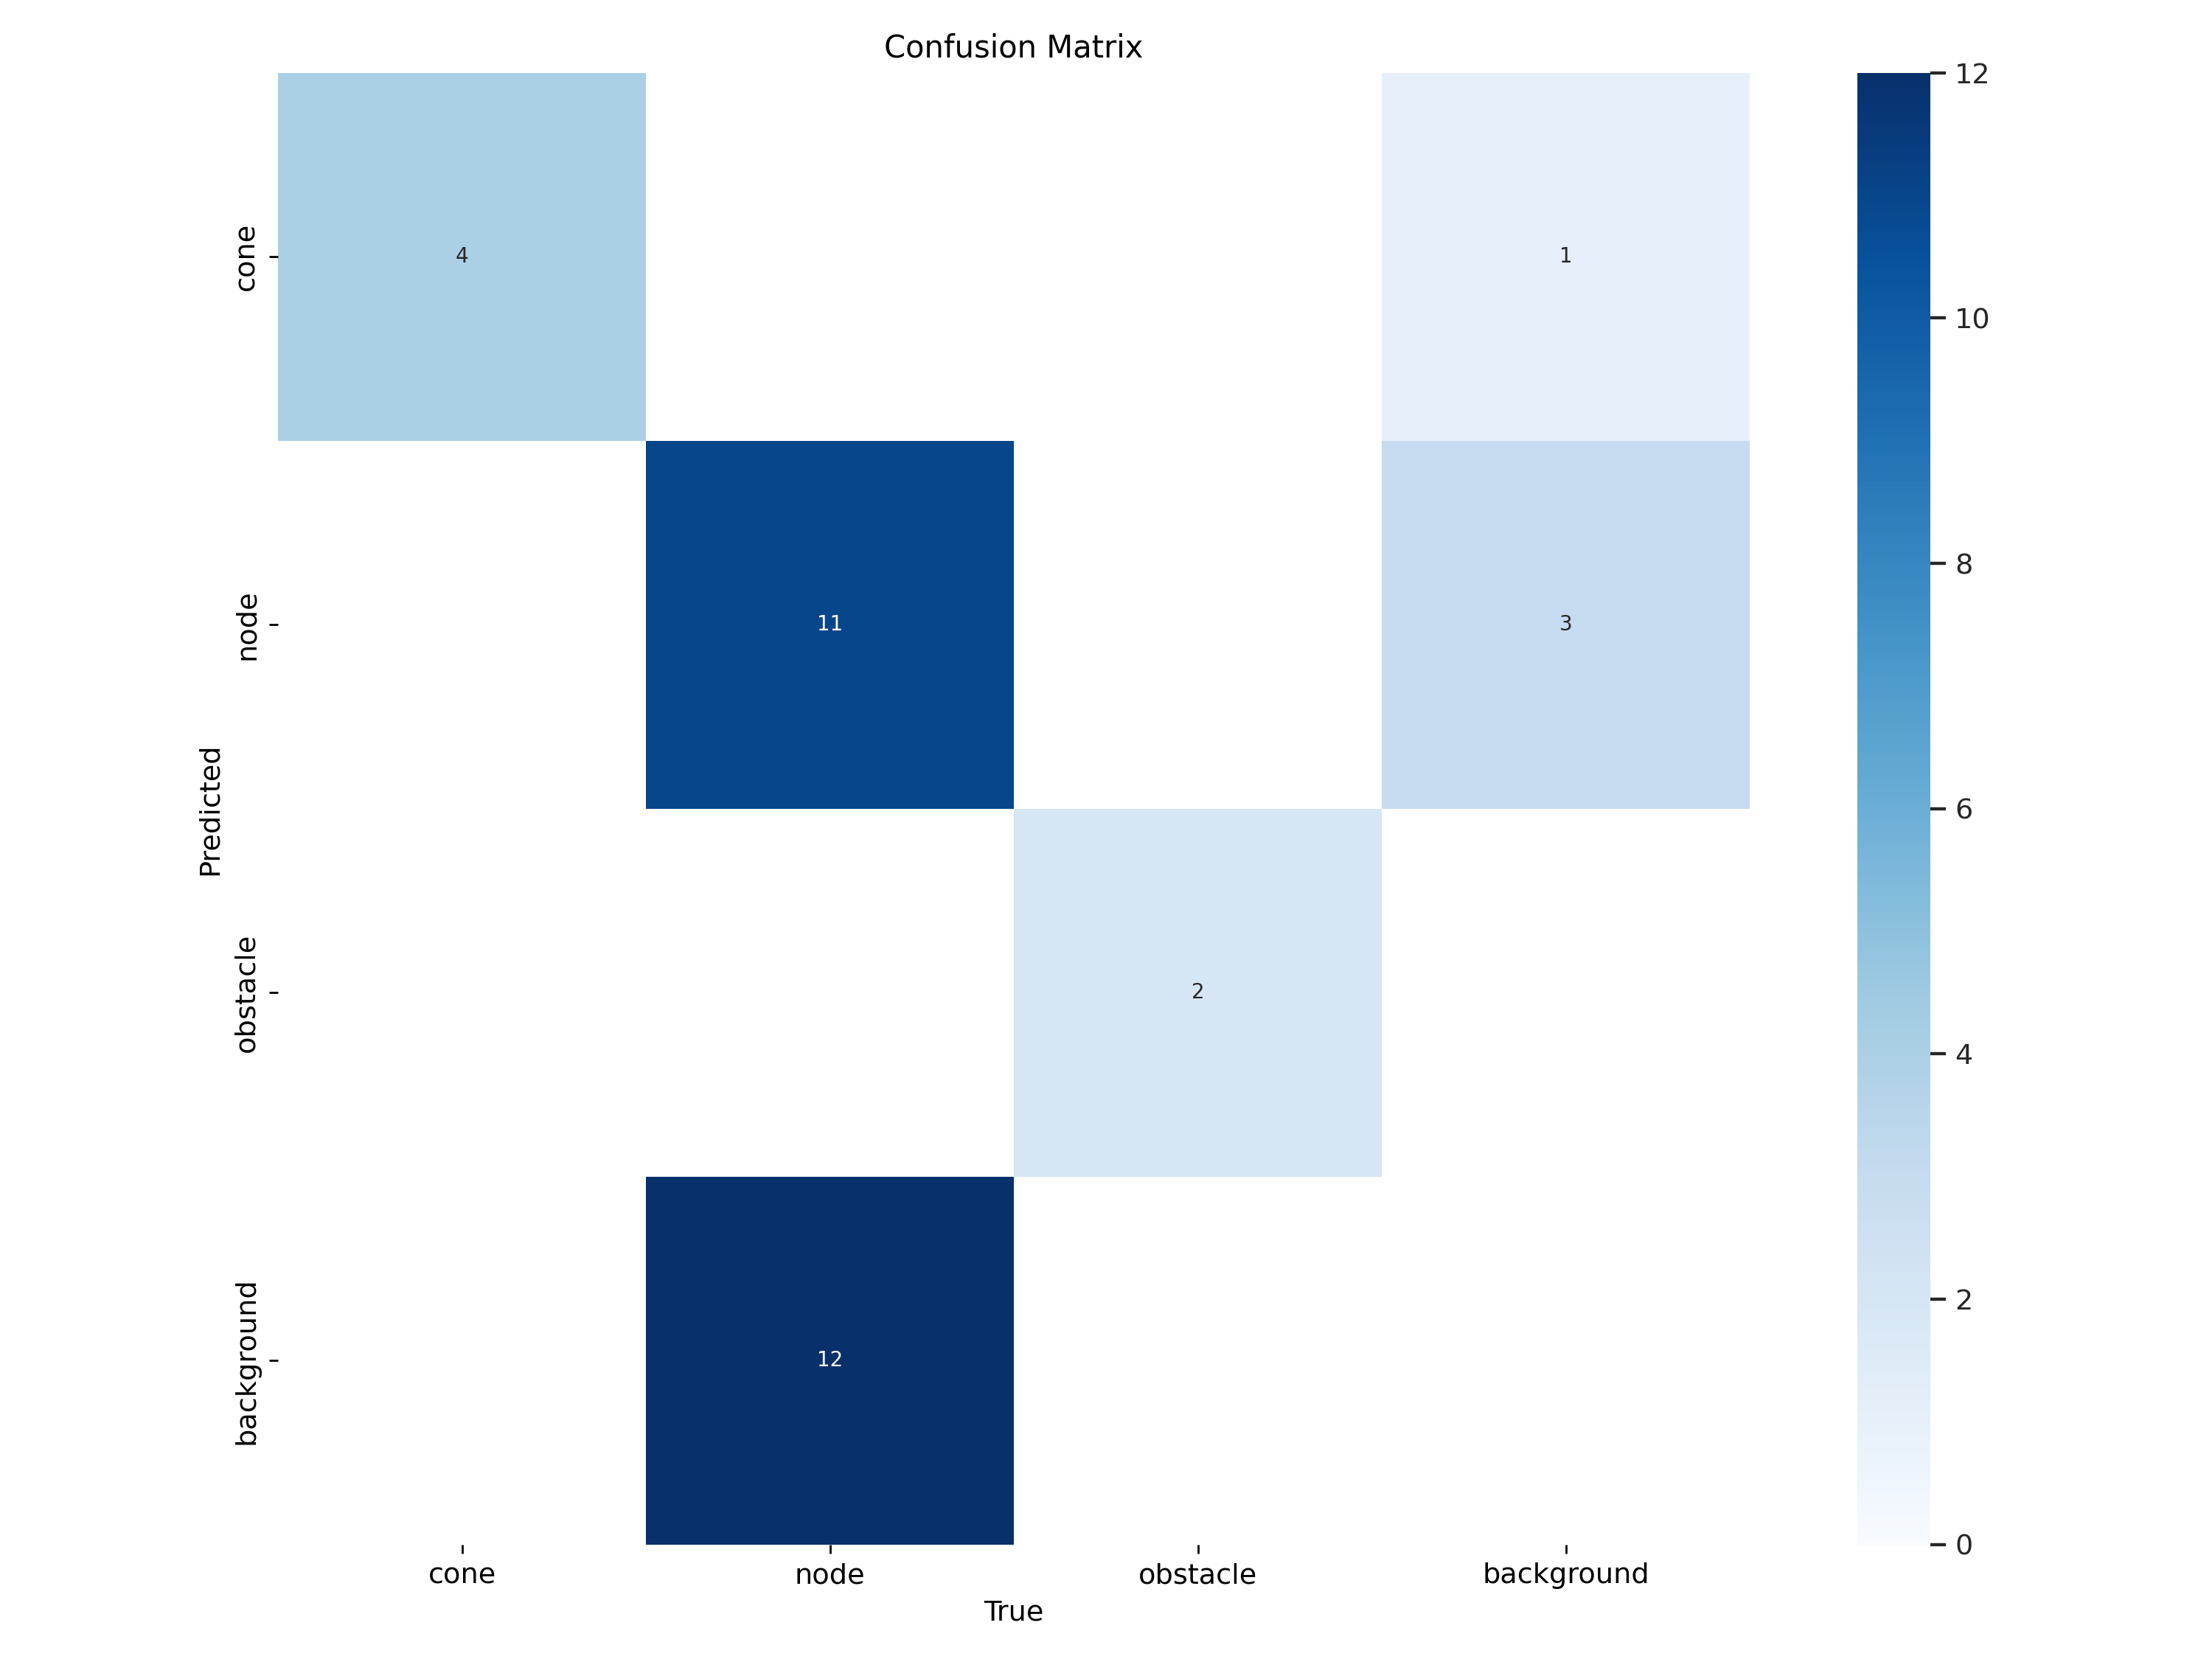
\includegraphics[width=\textwidth -20mm]{assets/informatik-prototyp/yolo/conf-matrix.png}
\caption{YOLOv11 Confusion Matrix}
\label{fig:conf-matrix-yolo}
\end{figure}

Aus dieser Matrix kann gelesen werden, dass alle Pylonen und alle Barrieren richtig erkannt werden. Einmal wird eine Pylone erkannt, obwohl es keine gibt. Die meisten vorausgesagten Knoten, sind wirklich Knoten, jedoch werden viele Knoten nicht erkannt. Dabei muss jedoch bedacht werden, dass es einfacher ist fuer das Model Knoten zu erkennen, die nahe und dadurch deutlicher sind und dass das Trainingsdatenset sehr klein ist. Trotzdem besteht ein sehr wahrscheinliches Risiko, dass ein Knoten nicht erkannt werden koennte.

TODO nur Barrieren \& Pylonen

\textbf{Fazit}
